\documentclass{article}
\usepackage[utf8]{inputenc}
\usepackage[T1]{fontenc}
\usepackage{graphicx}
\usepackage{hyperref}
\usepackage{geometry}
\geometry{margin=1in}

\title{AMIDA}
\date{Encyclopaedia Britannica (1771)}

\begin{document}
\maketitle

\section*{Historical source}
\textbf{Entry ID:} \texttt{entry-amida-560} \\
\textbf{Volume ID:} 191253801 \\
\textbf{Character Count:} 1171

\subsection*{Extracted Text}
AMIDA, a god worshipped by the japané, who has many temple credited to him in the island of Japan, of which the principal is at Jedo. The Japanese have fuch a confidence in their laid Andanda, that they hope to train several filing by the frequent invoces into one of the same. One of the figures of this idol is reprefeated at Rome.

Amida (une groge), a principal city of Méopomisnia (Libre Notias) y'\_Amanda\_ (Polandry); frutated on a high mountain, on the beaches of Afyrits, on the Yrys, you ever receive the Symphian— It was taken from the Romans in the time of the emperor Conflars, by Scarye Ring of Perita. The logic is fold to have call him 20.00 men, however, he reduced it to fuch ruin, that the emperor afterwards wept over it. According to Jamaimia Macrellana, the city may reside, like chiff offers were crucified; and the refl, with the soldiers and inhabitants, either put to the foreword or carried into registry, except our billionam landlir, and two orthree more, who, in the dead of the night, escaped through a polsum upterced by the enemy. The inhabits of Zollibs, however, being obliged to leave than own city by Jovian’s treaty with ACT [ 97] ACT



\section*{Source record}
\begin{itemize}
\item \textbf{Dataset:} \texttt{NationalLibraryOfScotland/encyclopaedia\_britannica\_illustrated}
\item \textbf{Dataset Revision:} \texttt{309f765b1ecc83e0a7f7762e44b4a927a7555443}
\item \textbf{Page ID:} \texttt{britannica:309f765b1ecc83e0a7f7762e44b4a927a7555443:train:560} \\
  \textbf{Filename:} \texttt{page-0560-c458f594fc79.jpg} \\
  \textbf{Row Index:} 560 \\
  \textbf{SHA256:} \texttt{c458f594fc79392e...}
\item \textbf{Page ID:} \texttt{britannica:309f765b1ecc83e0a7f7762e44b4a927a7555443:train:563} \\
  \textbf{Filename:} \texttt{page-0563-d12ce09577cd.jpg} \\
  \textbf{Row Index:} 563 \\
  \textbf{SHA256:} \texttt{d12ce09577cd595f...}
\end{itemize}

\begin{figure}[h]
\centering
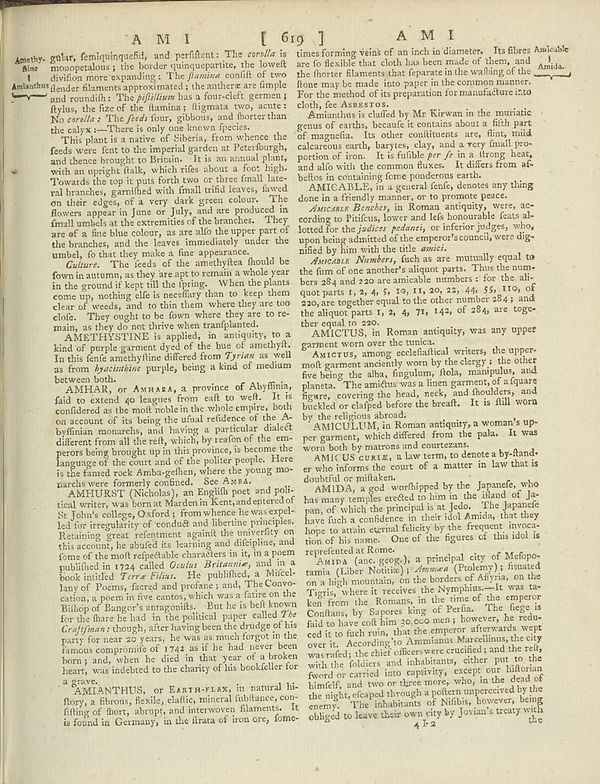
\includegraphics[width=0.85\textwidth]{../scans/page-0560-c458f594fc79.jpg}
\caption*{Source scan: \texttt{page-0560-c458f594fc79.jpg}}
\end{figure}
\begin{figure}[h]
\centering
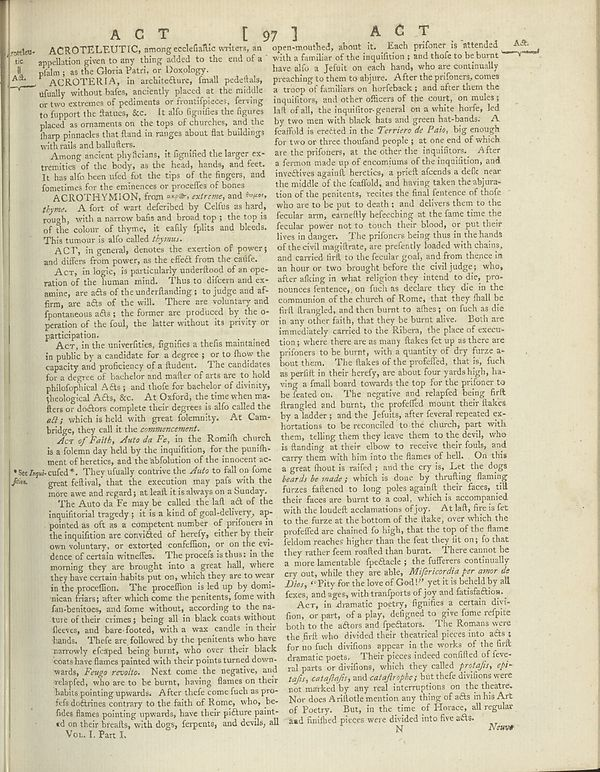
\includegraphics[width=0.85\textwidth]{../scans/page-0563-d12ce09577cd.jpg}
\caption*{Source scan: \texttt{page-0563-d12ce09577cd.jpg}}
\end{figure}

\end{document}
